\documentclass{article}

\usepackage{lipsum}
\usepackage[margin=2cm, left=2cm, includefoot]{geometry}
\usepackage{graphicx}
\usepackage{float}
\usepackage{hyperref}

% Header and footer
\usepackage{fancyhdr}
\pagestyle{fancy}

\rhead{}
\lhead{}
\fancyfoot{}
\fancyfoot[R]{\thepage}
\renewcommand{\headrulewidth}{0pt}
\renewcommand{\footrulewidth}{0pt}
%

\begin{document}

\begin{titlepage}
	\begin{center}
		\line(1,0){400}\\
		[6mm]
		\huge{\bfseries PROJECT TENDER}\\
		[2mm]
		\line(1,0){400}\\
		[5mm]
		\large\textbf{PROJECT:}\\\textsc{Financial Markets Simulation with Multiple Competing Algorithmic Trading Entities}\\
		[3mm]
		\large\textbf{CLIENT:}\\\textsc{Adrian Wilford}\\
		[3mm]
		\large \textbf{TEAM:}\\\textsc{Funge}\\
		\line(1,0){400}\\
		[5mm]
		\large \textbf{Team Members:}\\
		[3mm]
		\large Matthew Botha\\
		\large Gian Paolo Buffo\\
		\large Matthias Harvey\\
        \large Dillon Heins\\[3mm]
		\begin{figure}[H]
			\centering
			\includegraphics[width=0.8\textwidth]{../teamPhoto.jpg}
			\caption{Matthew Botha, Matthias Harvey, Gian Paolo Buffo, Dillon Heins}
		\end{figure}
    \end{center}

    \begin{flushright}
        \textsc{\large Department of Computer Science\\
        University of Pretoria\\
        01 May 2016\\}
    \end{flushright}
\end{titlepage}

\section{The Team}
	\subsection{Matthew Botha}
		
	\subsection{Matthew Botha}
		\textbf{Profile:}\\
		I am fascinated by all things technological and love tinkering with new gadgets and technology. I am interested in artificial intelligence, especially in computer security systems, as well as computer networks and the Internet of Things. I am an avid reader and enjoy cooking and playing guitar.
		\subsubsection{Contact}
			\begin{itemize}
				\item \href{mailto:m.botha41@gmail.com}{\textbf{Email} m.botha41@gmail.com}
				\item \href{https://github.com/MatthewBotha}{\textbf{Github} MatthewBotha}
			\end{itemize}
		\subsubsection{Photo}
		\begin{figure}[H]
			\centering
			
\includegraphics[width=250px]{../Matt.jpg}
			\caption{Matthew Botha}
		\end{figure}
		\subsubsection{Interests}
		\begin{itemize}
			\item New and emerging technologies
			\item Computer security, artificial intelligence, networks and programming.
			\item Literature
			\item Mathematics
		\end{itemize}
		
\subsubsection{Technical Skills}
			\begin{tabular}{| l | l | l |}
				Java   & C		& NASM                        \\
				Git    & C++      & Haskell                     \\
				SQL    & C\#	& HTML, CSS, JavaScript, PHP   \\
				Django & Unity3D	& Python	
			\end{tabular}
		
\subsubsection{Past Experience \& Achievements}
			\begin{itemize}
				\item \textbf{Past Experience}
				\begin{itemize}
					\item Web Developer for Ms. Vreda Pieterse (Software engineering lecturer)
					\begin{itemize}
						\item University of Pretoria
						\item July 2014 - Present
					\end{itemize}
					\item Teaching Assistant
					\begin{itemize}
						\item University of Pretoria
						\item August 2015 - Present
					\end{itemize}
					\item Developer at Monkey \& River during 2015
					\begin{itemize}
						\item Pretoria
						\item Helped develop a web-based system (using ASP.NET MVC) to compare municipalities and districts in SA. See demo here: \href{http://salgabarometerdemo.org.za/RatingTool}{RatingTool}
						\item June 2015 - December 2015
					\end{itemize}
				\end{itemize}
				
				\item \textbf{Achievements}
				\begin{itemize}
					\item Deputy Head Boy
					\begin{itemize}
						\item Hatfield Christian School
						\item 2013
					\end{itemize}
					\item Currently working on a team developing a web-based peer review system for the University of Pretoria
				\end{itemize}
			\end{itemize}
		\subsubsection{Non-technical Skills}
			\begin{itemize}
				\item Enjoys challenges
				\item Always looking to learn
				\item Works well in teams
				\item Fast at learning new technologies
				\item Adaptable to change
			\end{itemize}
		\subsubsection{Hobbies}
			\begin{itemize}
				\item Cooking
				\item Reading
				\item Hiking
				\item Dungeon Master (D\&D 5e, Fantasy AGE, W40k Rogue Trader, Numenera)
			\end{itemize}
		\subsubsection{Motivation for Choosing Project}
		
			
	\cleardoublepage		
		
	\subsection{Gian Paolo Buffo}
		\textbf{Profile:}\\
	My favourite part about software development is being able to blend creativity and functionality to create efficient, interactive and engaging software. I am most interested in multimedia software implementations, where the user experience comes above all else. In my spare time I like to go hiking or geek it out with a good book, videogame or boardgame.  
	\subsubsection{Photo}
		\begin{figure}[H]
			\centering
			
\includegraphics[width=0.6\textwidth]{../gianpaolo.jpg}
			\caption{Gian Paolo Buffo}
		\end{figure}
	\subsubsection{Contact}
		\begin{itemize}
			\item \href{mailto:gpbuffo@gmail.com}
				{\textbf{Email} gpbuffo@gmail.com}
			\item \href{https://github.com/GianPaoloBuffo}
				{\textbf{Github} GianPaoloBuffo}
			\item \href{https://www.linkedin.com/in/gpbuffo}
				{\textbf{LinkedIn} gpbuffo}
		\end{itemize}
	\subsubsection{Interests}
		\begin{itemize}
			\item Computer Graphics
			\item Computer Networks
			\item Web Development
			\item Videogame Theory, Design and Development
			\item Creative Writing
		\end{itemize}
	\subsubsection{Technical Skills}
		\begin{tabular}{| l | l | l |}
			C++		& HTML5, CSS, JavaScript, PHP	& WebGL    	\\
			Java    & NASM     	& AngularJS							\\
			Git 	& SQL     	& C\#									\\
			Unity3D & Adobe Photoshop, Flash, After Effects &                  
		\end{tabular}
	\subsubsection{Past Experience \& Achievements}
		\begin{itemize}
			\item \textbf{Past Experience}
			\begin{itemize}
				\item Teaching Assistant - Multimedia
				\begin{itemize}
					\item University of Pretoria
					\item February 2015 - June 2015
				\end{itemize}
				\item Teaching Assistant - Computer Science
				\begin{itemize}
					\item University of Pretoria
					\item June 2015 - Present
				\end{itemize}
				\item Assistant - Visual Design
				\begin{itemize}
					\item University of Pretoria
					\item February 2016 - Present
				\end{itemize}
			\end{itemize}
			\item \textbf{Achievements}
				\begin{itemize}
					\item Dux Scholar (highest grade average) for 4 consecutive years in High School
					\item Valedictorian Speaker
					\item Top achievers' award for BIS Multimedia: 2014 \& 2015
					\item Overall distinction: 2014 \& 2015
					\begin{itemize}
						\item 82.39\% cumulative average
					\end{itemize}
					\item Golden Key International Honour Society member
				\end{itemize}
		\end{itemize}
	\subsubsection{Non-technical Skills \& Hobbies}
		\begin{itemize}
			\item Non-technical Skills
			\begin{itemize}
				\item Willingness to learn
				\item Solid presentational skills
				\item Good work ethic and team dynamics
			\end{itemize}
			\item Hobbies
			\begin{itemize}
				\item Hiking
				\item Writing
				\item Digital and board gaming
			\end{itemize}
		\end{itemize}
		\subsubsection{Motivation for Choosing Project}
		The inherent nature of this project means that I will not only be challenged in terms of the application of my Computer Science knowledge, but I will also be exposed to a new field of trade, financial markets and the economy.
\\\\
This project will, above all else, provide a valuable learning experience and the finished system is one that can be applied in real-world situations. The project scope is clear and the client is well-known in the industry. 

	\cleardoublepage

	\subsection{Matthias Harvey}
			\textbf{Profile:}\\
	I have a passion for mathematics, science and software development. My special interests are computer graphics, simulations and artificial intelligence. I thrive on challenging projects. In my spare time I study French and Japanese, love music and play the guitar.
	\subsubsection{Contact}
	\begin{itemize}
		\item \href{mailto:matthiasharvey@gmail.com}{\textbf{Email} matthiasharvey@gmail.com}
		\item \href{https://github.com/MatthiasHarvey}{\textbf{Github} MatthiasHarvey}	
		\item \href{https://za.linkedin.com/in/matthias-harvey-68b30995}{\textbf{LinkedIn} Matthias Harvey}
	\end{itemize}
	\subsubsection{Photo}
	\begin{figure}[H]
		\centering
		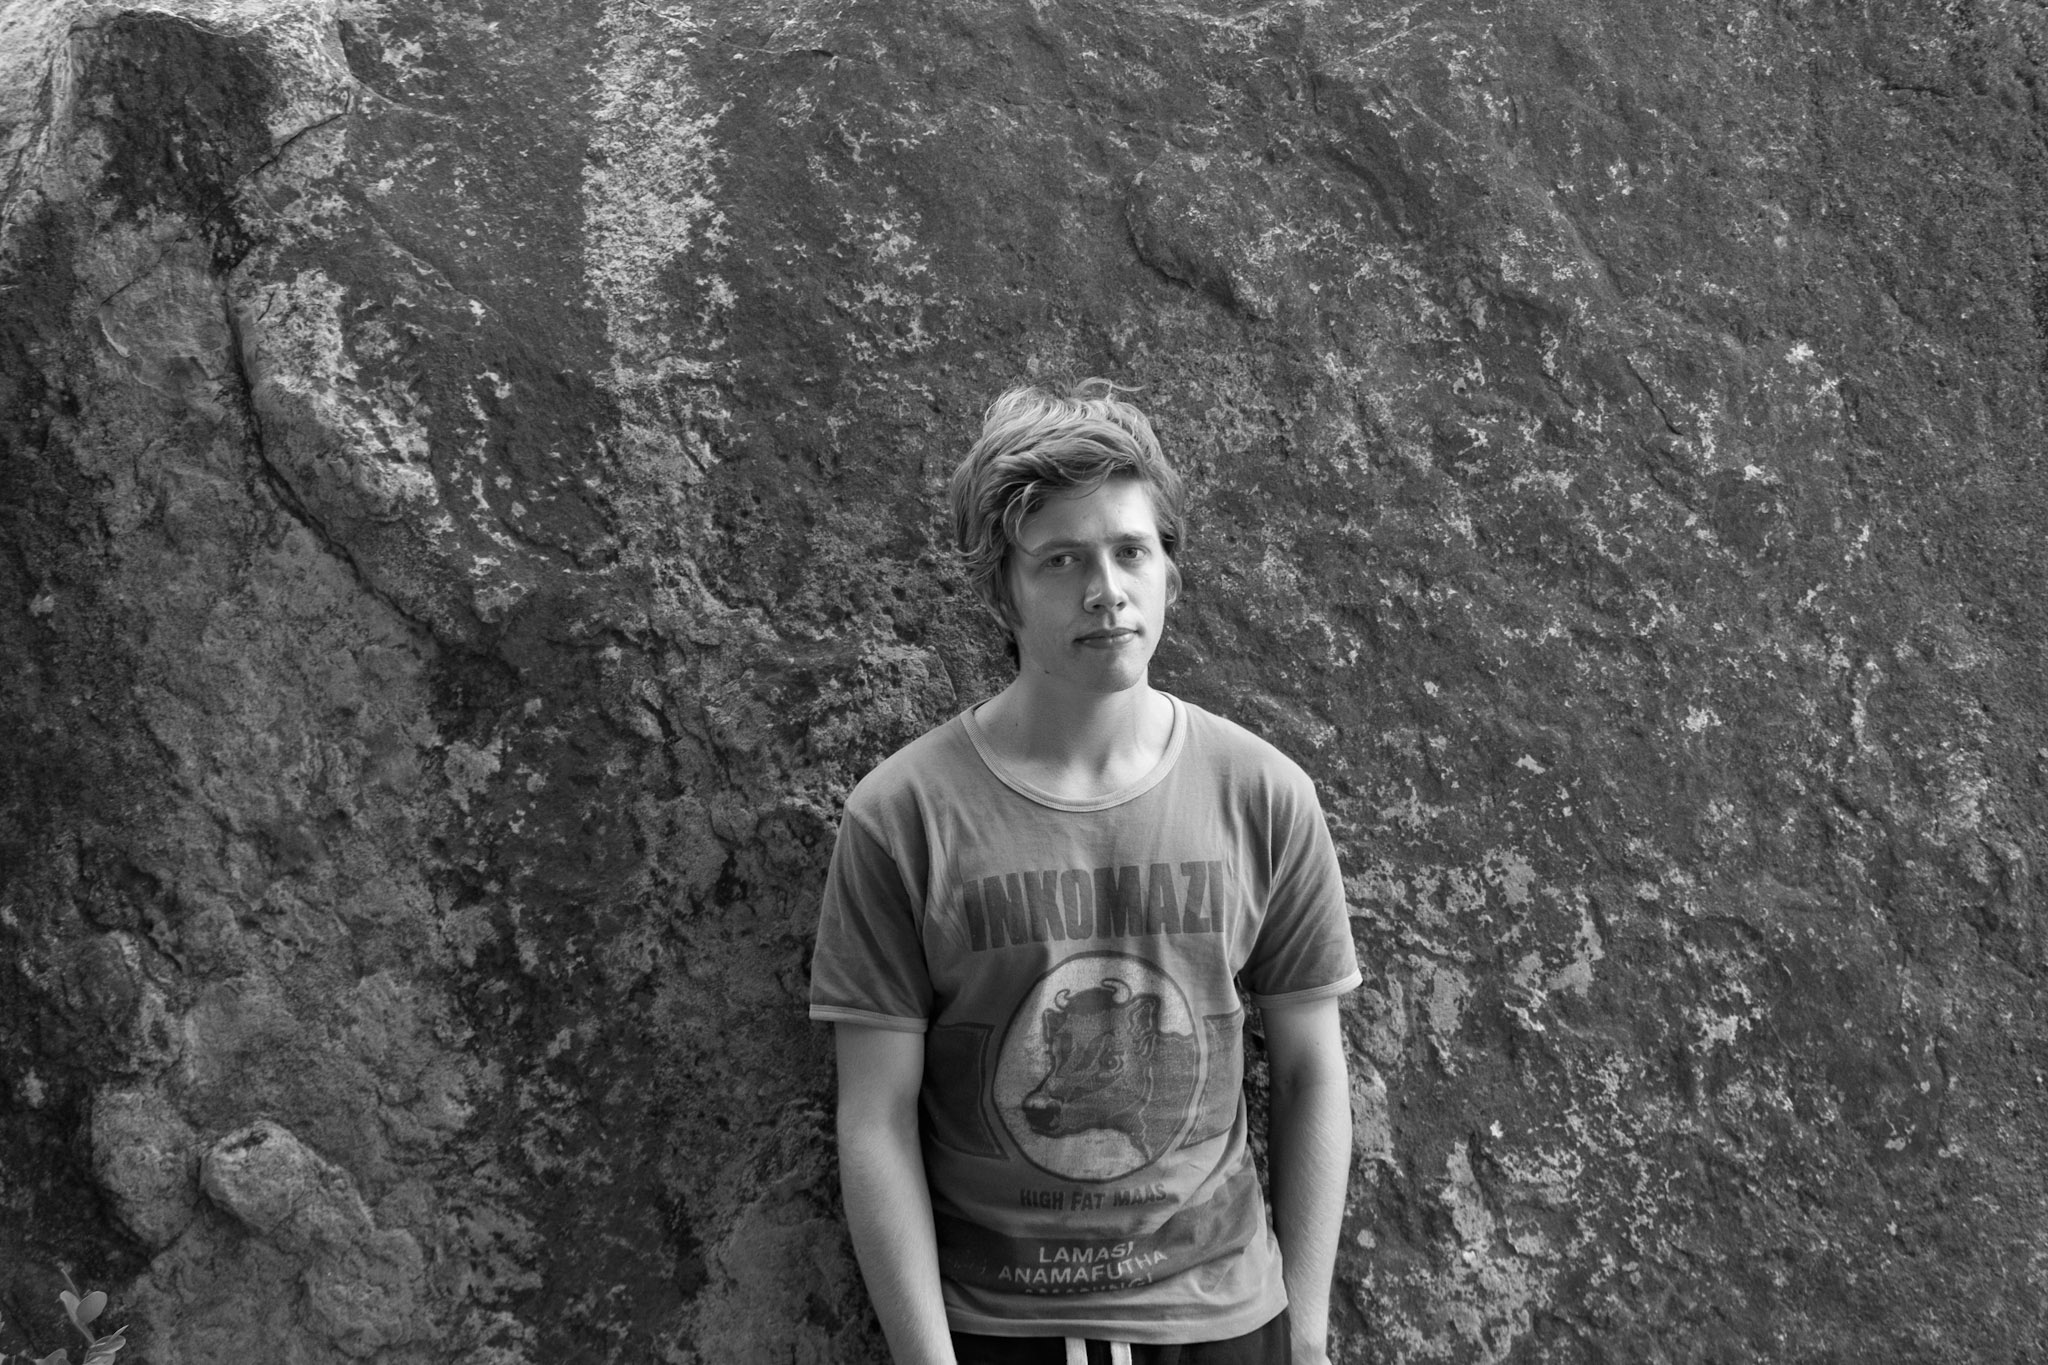
\includegraphics[width=0.7\textwidth]{../matthias.jpg}
		\caption{Matthias Harvey}
	\end{figure}
	\subsubsection{Interests}
	\begin{itemize}
		\item Computer graphics, artificial intelligence, game programming, simulations
		\item Mathematics
		\item Physics
		\item French - read, write. Speak - intermediate. Japanese – beginner
	\end{itemize}
	\subsubsection{Technical Skills}
	
	\begin{tabular}{| l | l | l |}
		Java   & C\#     & F\#                          \\
		Git    & C++, NASM     & Haskell                     \\
		OpenGL & SQL     & HTML, CSS, JavaScript, PHP   \\
		Django & Unity3D & Python                     
	\end{tabular}

	\subsubsection{Past Experience \& Achievements}
	\begin{itemize}
		\item \textbf{Past Experience}
		\begin{itemize}
			\item Research Assistant for the SSFM Research Group
			\begin{itemize}
				\item University of Pretoria
				\item Assisting Prof. S. Gruner and Dr. N. Timm with research pertaining to Formal Methods - specifically 3-Valued Bounded Model Checking
			\end{itemize}
			\item Web Developer for Ms. Vreda Pieterse (Software engineering lecturer)
			\begin{itemize}
				\item University of Pretoria
				\item July 2014 - Present
			\end{itemize}
			\item Teaching Assistant
			\begin{itemize}
				\item University of Pretoria
				\item February 2015 - Present
			\end{itemize}
			
			\item Developer at Monkey \& River during 2015
			\begin{itemize}
				\item Pretoria
				\item Helped develop a web-based system (using ASP.NET MVC) to compare municipalities and districts in SA. See demo here: \href{http://salgabarometerdemo.org.za/RatingTool}{RatingTool}
				\item June 2015 - December 2015
			\end{itemize}
			
			\item Intern at Agnomen Design
			\begin{itemize}
				\item Agnomen Design. An indie-game studio based in Cape Town
				\item $ \pm 3 $ months experience during holidays since 2014
			\end{itemize}
		\end{itemize}
		
		\item \textbf{Achievements}
		\begin{itemize}
			\item High school science expo – silver at nationals (Electricity from cardboard)
			\item Completed an online course: Creative Coding (from Monash University) 2014
			\item Placed 5th at the national finals of the Standard Bank IT Challenge 2015
			\item Currently team leader of six selected students developing a web-based peer review system for the University of Pretoria
			\item Invited to Golden Key
			\item Distinction average throughout university
		\end{itemize}
	\end{itemize}
	
	\subsubsection{Non-technical Skills/Hobbies}
	\begin{itemize}
		\item Rock Climbing, parkour, mountain biking
		\item Guitar, music production
		\item Computer generated art through coding
	\end{itemize}
		\subsubsection{Motivation for Choosing Project}
		This will be a very fun and challenging project. I have had a growing interest in financial market simulations for a while now, so this is a perfect opportunity for us to learn more about them.\\
		
		I am very interested in creating artificial intelligence that can do this type of analysis - I have been wanting to do this since last year, and was going to start doing this anyway so it would be great to do it for a company that can advise and guide us.\\

		Our recent lectures in AI have really inspired me, and I am excited to get my feet wet, especially dabbling with trade algorithms involving AI.
	\cleardoublepage
	
	\subsection{Dillon Heins}
		\subsubsection{Motivation for Choosing Project}

\cleardoublepage
    
\section{Project Execution}
	\subsection{Development Methodology}
	We intend to follow the Scrum approach to Agile software development throughout the course of project development. Agile itself is not a methodology and does not provide concrete steps which we would be able to follow. Hence we have opted to incorporate Scrum-specific methods within the Agile movement. The reasons we have considered to use this methodology are as follows:
		\begin{itemize}
			\item The agile approach ensures that we as a team will be able to respond effectively and efficiently to unpredictability through incremental, iterative sprints
			\item These short sprints enable us to ensure that the product is kept in a potentially shippable state at all times
			\begin{itemize}
				\item This is effective as it ensures the product is always integrated and tested
				\item By having these short sprints of development it will enable us to periodically demonstrate our product to the client so that we are able to receive feedback, adapt to said feedback and plan accordingly for the next sprint
			\end{itemize}
			\item Scrum and agile work well together as Scrum is simple and flexible
			\item Scrum enables test-driven development
			\item Agile incorporates both the business and technical side and enables all involved with the project to engage and function together
			\begin{itemize}
				\item Scrum only has three roles: Product owner, Team, and Scrum Master
				\item These roles bode well to the nature of this project
			\end{itemize}
			\item To summarise: Scrum emphasises "empirical feedback, team self management, and striving to build properly tested product increments within short iterations"
			\begin{itemize}
				\item This ensures the continuous act of inspecting and adapting in order to deal with complexity and risk
				\item Our team is responsible for self management which enables us to function well without having to have continuous contact with our client
				\item Scrum decision-making revolves around real-world situations and feedback rather than assumption
			\end{itemize}
		\end{itemize}
	\subsection{Methods of Informing Client}
	At the moment our team has communication lines set up using:
		\begin{itemize}
			\item Slack - integrated with GitHub
			\item Telegram
		\end{itemize}
		We plan to use Slack as a formal means of communicating our project's progress. If you'd like, we can then add you, as the client, to our Slack group so that we are able to continuously communicate with you.\\\\
		Slack enables one to create channels and therefore you, as the client, would be able to choose whether you want to join our general channel to view general conversation and progress or we could create another channel on which we periodically post important information and progress as well as ask for your feedback.\\\\
		If you, as the client, feel it is necessary we can schedule periodic video call sessions in order to discuss our progress and receive feedback.\\\\
		In general though we are very flexible and no matter the platform the client prefers we will ensure to keep you continuously updated as well as ask for and implement any feedback.
	\subsection{Initial Ideas for Solving Technical Challenges}
	Functional programming could be used to solve the concurrent, and algorithmic challenges.
	\begin{itemize}
		\item The expressiveness of functional programming is a major benefit as this will allow us to write the algorithms in a very clear and concise manner.
		\item Testing is made easier and more definite in a functional language as you have pure functions without side-effects.
		\item The thread-safe nature of functional programming is perfect for the concurrent needs of the system.
	\end{itemize}

	\subsection{Possible Technologies to Use for Project}
	.NET would be our go-to choice for technology since we could use the functional language F\# and combine it with C\# code and libraries if needed. F\# is really powerful and succinct, and combines functional programming with the best aspects of Object-Orientated programming. \\

	Correctness of the software is obviously a concern as a mistake in the code could cause a lot of money to be lost. The succinctness and static typing of F\# helps greatly with this, as it is much easier to reason about strongly typed, clear and well-written code.\\

	A great type system and/or DSL (domain specific language) can be created within F\# to assist in the development and verification of the system.\\

	The other great thing about the type system is that you can catch most bugs at compile time, rather than getting unwanted surprises at runtime. \\

	Here is some example F\# code that analyses stock markets: \href{http://www.tryfsharp.org/Learn/financial-computing#analyzing-stock-markets}{TryF\# - Analysing Stock Markets}

	\subsection{Final Deliverable}
	As specified in the proposal.

\end{document}
